\section{Applications Téléphoniques}
\author{Kévin Moreau}


\begin{frame}
	\frametitle{Les différentes fonctionnalités à ajouter}

	\begin{block}{Les fonctionnalités}
	 \begin{itemize}
      \item Réécriture de numéro ;
	  \item Click2Call ;
	  \item Appel depuis l'historique Dynamease;
	  \item Transfert d'appel.
	 \end{itemize}
	\end{block}
\end{frame}

\begin{frame}
	\frametitle{Réécriture du numéro (1/4) : Cahier des charges}

	\begin{block}{Étude du cahier des charges}
	 \begin{itemize}
      \item Utilisation d'un Trunk ;
      \item Redirection des appels de l'utilisateur Dynamease ;
      \item Utilisable uniquement pour les utilisateurs Privilège.
	 \end{itemize}
	\end{block}
\end{frame}

\begin{frame}
	\frametitle{Réécriture du numéro (2/4) : Communication des différents services}

	\begin{center}
	  \begin{figure}
        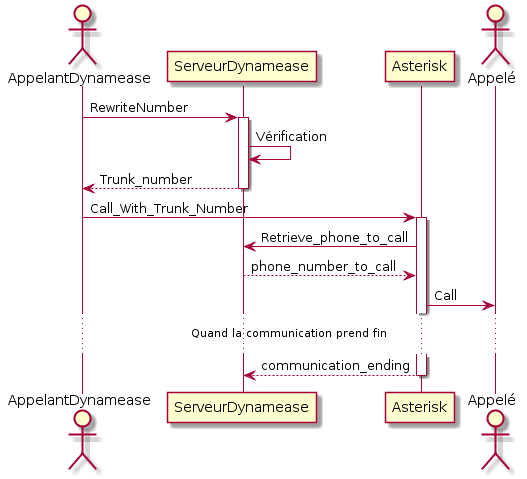
\includegraphics[scale=0.30]{images/sequence_rewirte.png}
	   \caption{Communication contextualisé}
	  \end{figure}
	\end{center}
\end{frame}

\begin{frame}
	\frametitle{Réécriture du numéro (3/4) : Traitement des requêtes envoyées par Asterisk}

	\begin{center}
	  \begin{figure}
        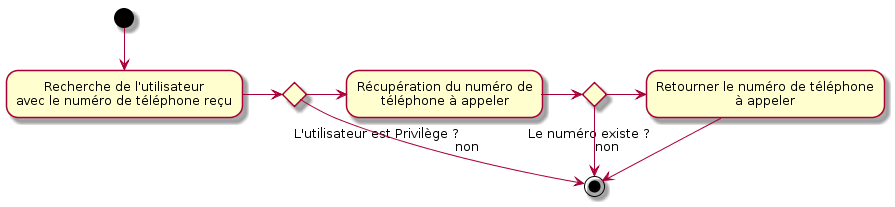
\includegraphics[scale=0.30]{images/activity_rewrite_ast.png}
	   \caption{Communication contextualisé}
	  \end{figure}
	\end{center}
\end{frame}

\begin{frame}
	\frametitle{Réécriture du numéro (4/4) : Traitement des requêtes envoyées par les applications téléphoniques}

	\begin{center}
	  \begin{figure}
        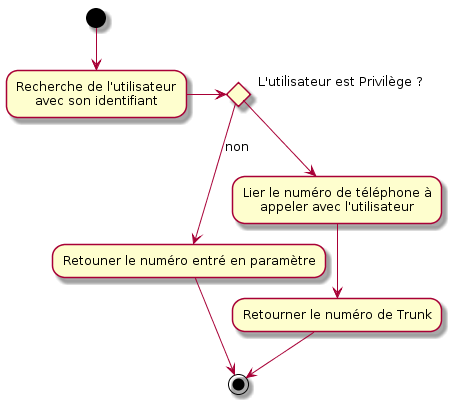
\includegraphics[scale=0.30]{images/activity_rewrite_app.png}
	   \caption{Communication contextualisé}
	  \end{figure}
	\end{center}
\end{frame}